\section{Шифр «Кузнечик»}\label{section-grig}\index{шифр!«Кузнечик»|(}
\selectlanguage{russian}

В июне 2015 года в России был принят новый стандарт блочного шифрования ГОСТ Р 34.12-2015~\cite{GOST-R:34.12-2015}. Данный стандарт включает в себя два блочных шифра -- старый ГОСТ 28147-89, получивший теперь название <<Магма>>, и новый шифр со 128 битным входным блоком, получившим название <<Кузнечик>>.

В отличие от шифра <<Магма>> новый шифр <<Кузнечик>> основан на SP-сети\index{SP-сеть} (сети замен и перестановок), то есть основан на серии обратимых преобразований, а не на ячейке Фейстеля\index{ячейка Фейстеля}. Как и другие популярные шифры, он является блочным раундовым шифром и имеет выделенную процедуру выработки раундовых ключей. Шифр работает с блоками открытого текста по 128 бит, а размер ключа шифра составляет 256 бит. Отдельный раунд шифра <<Кузнечик>> состоит из операции наложения ключа, нелинейного и линейного преобразований, как изображено на рис.~\ref{fig:kuznechik-step}. Всего в алгоритме 10 раундов, последний из которых состоит только из операции наложения ключа. 

\begin{figure}[htb]
	\centering
	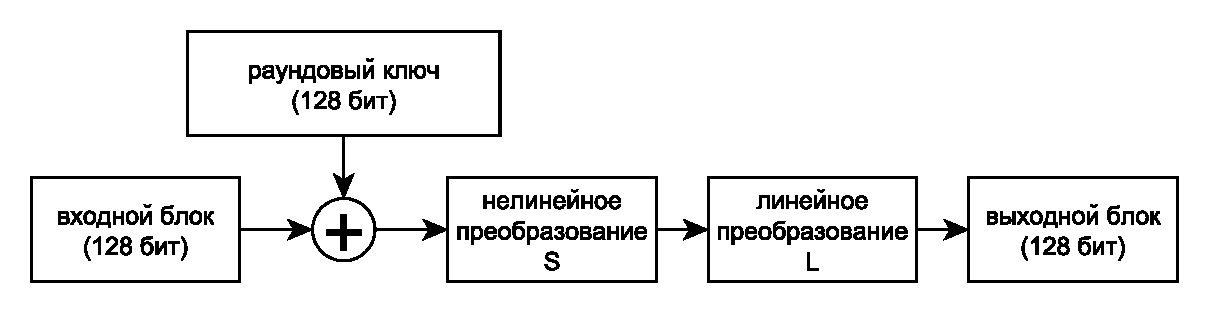
\includegraphics[width=0.8\textwidth]{pic/kuznechik-step}
  \caption{Один раунд шифрования в алгоритме <<Кузнечик>>}
  \label{fig:kuznechik-step}
\end{figure}

Нелинейное преобразование $S$ разбивает блок данных из 128 бит на 16 блоков по 8 бит в каждом, как показано на рис.~\ref{fig:kuznechik-s}.

\begin{figure}[htb]
	\centering
	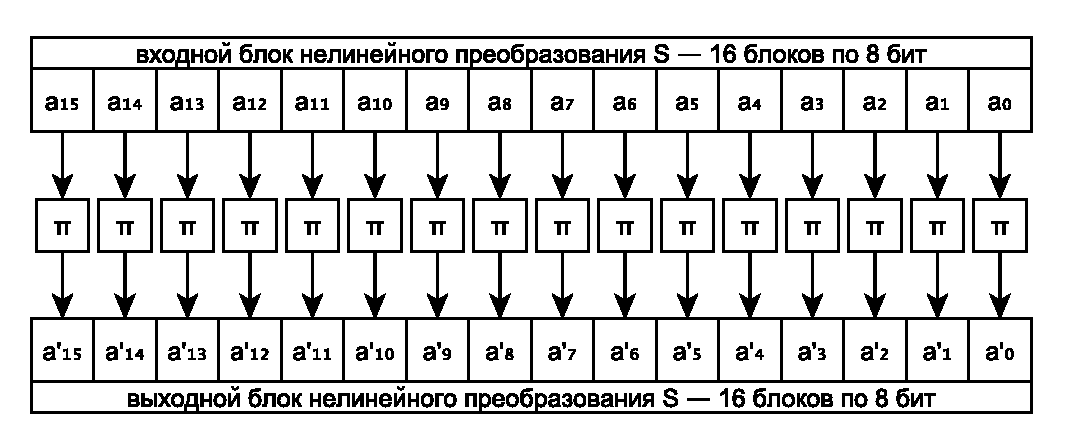
\includegraphics[width=0.9\textwidth]{pic/kuznechik-s}
  \caption{Нелинейное преобразование $S$ в алгоритме <<Кузнечик>>}
  \label{fig:kuznechik-s}
\end{figure}

Каждый из 8-ми битных блоков $a$ трактуется как целое беззнаковое число $\text{Int}_8 a$ и выступает в качестве индекса в заданном массиве констант $\pi'$. Значение по индексу $\text{Int}_8 a$ в массиве констант $\pi'$ обратно преобразуется в двоичный вид и выступает в качестве одного из 16 выходных блоков нелинейного преобразования $S$.

\begin{quote}\noindent {\scriptsize$\pi'$ = (252, 238, 221, 17, 207, 110, 49, 22, 251, 196, 250, 218, 35, 197, 4, 77, 233, 119, 240, 219, 147, 46, 153, 186, 23, 54, 241. 187, 20, 205, 95, 193, 249, 24, 101, 90, 226, 92, 239, 33, 129, 28, 60, 66, 139, 1, 142, 79, 5, 132, 2, 174, 227, 106, 143, 160, 6, 11, 237, 152, 127, 212, 211, 31, 235, 52, 44, 81, 234, 200, 72, 171, 242, 42, 104, 162, 253, 58, 206, 204, 181, 112, 14, 86, 8, 12, 118, 18, 191, 114, 19, 71, 156, 183, 93, 135, 21, 161, 150, 41, 16, 123, 154, 199, 243, 145, 120, 111, 157, 158, 178, 177, 50, 117, 25, 61, 255, 53, 138, 126, 109, 84, 198, 128, 195, 189, 13, 87, 223, 245, 36, 169, 62, 168, 67, 201, 215, 121, 214, 246, 124, 34, 185, 3, 224, 15, 236, 222, 122, 148, 176, 188, 220, 232, 40, 80, 78, 51, 10, 74, 167, 151, 96, 115, 30, 0, 98, 68, 26, 184, 56, 130, 100, 159, 38, 65, 173, 69, 70, 146, 39, 94, 85, 47, 140, 163, 165, 125, 105, 213, 149, 59, 7, 88, 179, 64, 134, 172, 29, 247, 48, 55, 107, 228, 136, 217, 231, 137, 225, 27, 131, 73, 76, 63, 248, 254, 141, 83, 170, 144, 202, 216, 133, 97, 32, 113, 103, 164, 45, 43, 9, 91, 203, 155, 37, 208, 190, 229, 108, 82, 89, 166, 116, 210, 230, 244, 180, 192, 209, 102, 175, 194, 57, 75, 99, 182).}\end{quote}

Линейное преобразование $L$ состоит из 16 операций линейного преобразования $R$, то есть $L = R^{16}$. Линейное преобразование $R$, в свою очередь, представляет блок из 128 бит как начальные значения 8-ми битовых ячеек регистра сдвига с линейной обратной связью (РСЛОС) с 16 ячейками, как показано на рис.~\ref{fig:kuznechik-p}. При сдвиге вычисляется сумма значений ячеек, домноженных на 16 констант. Значения ячеек и константы трактуются как элементы поля Галуа $GF(2^8)$ с модулем $p(x) = x^8 + x^7 + x^6 + x + 1$ (см. раздел~\ref{section-fields}), умножение и сложение также проходят в этом поле.

\begin{figure}[htb]
	\centering
	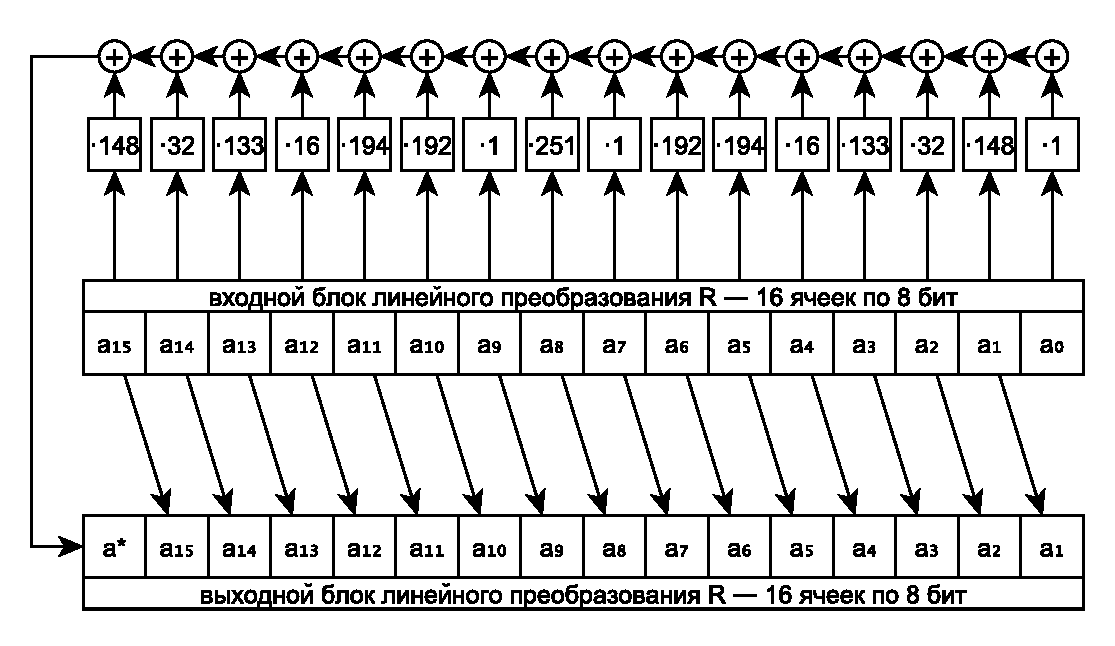
\includegraphics[width=0.9\textwidth]{pic/kuznechik-p}
  \caption{Линейное преобразование $R$ в алгоритме <<Кузнечик>>}
  \label{fig:kuznechik-p}
\end{figure}

Алгоритм развёртывания ключа основан на ячейке Фейстеля, хотя и не использует её ключевую особенность (обратимость). Начало алгоритма изображёно на рис.~\ref{fig:kuznechik-keys}.

\begin{figure}[htb]
	\centering
	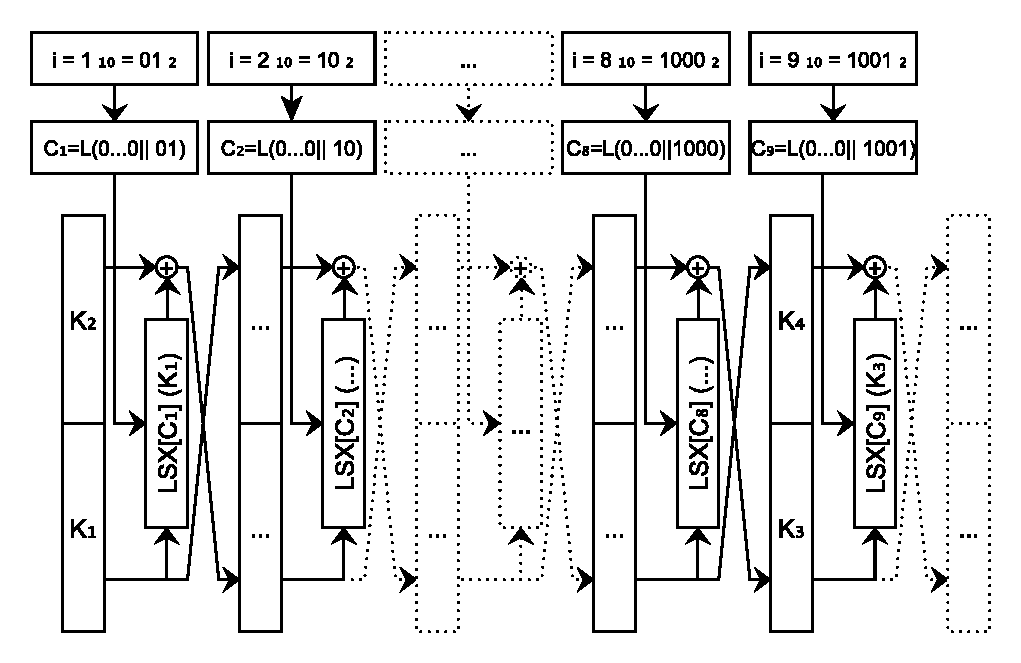
\includegraphics[width=0.90\textwidth]{pic/kuznechik-keys}
  \caption{Часть алгоритма развёртывания ключа в <<Кузнечике>>}
  \label{fig:kuznechik-keys}
\end{figure}

\begin{itemize}
	\item Целые числа $i$ от 1 до 32 представляются в виде двоичных векторов по 128 бит. К каждому из них применяется линейное преобразование $L=R^{16}$ как было описано ранее. Получаются 32 константы $C_{1}...C_{32}$.
	\item Первые два раундовых ключа $K_1$ и $K_2$ получаются разбиением мастер-ключа $K$ (256 бит) на два блока по 128 бит каждый.
	\item Следующая пара раундовых ключей $K_3$ и $K_4$ получается из первой пары $K_1$ и $K_2$ применением 8 раундов ячейки Фейстеля. В качестве функции Фейстеля, преобразующую один из блоков на каждом раунде, выступает преобразование $\text{LSX}(C_i), i=1,\dots,8$. То есть (читая справа налево, как принято с операторами) побитовое сложение с заданной константой $C_i$, а потом нелинейное и линейное преобразования $S$ и $L$, как они были описаны ранее.
	\item Все остальные пары раундовых ключей вплоть до $K_{9}$ и $K_{10}$ получаются аналогичным образом, используя предыдущую пару ключей и по 8 констант $C_i$.
\end{itemize}

Так как и легальный отправитель, и легальный получатель используют функцию развёртывания ключа в прямом направлении, начиная с пары $K_1, K_2$ и до $K_{9}, K_{10}$, то алгоритм никогда не <<идёт назад>> и не использует ключевую особенность ячейки Фейстеля -- её обратимость.

В отличие от стандарта 1989 года, в текст нового стандарта не стали включать режимы сцепления блоков, а вынесли это в отдельный ГОСТ Р 34.13-2015 <<Режимы работы блочных шифров>>~\cite{GOST-R:34.13-2015}.

В работе 2015 года Бирюков, Перрин и Удовенко (\langen{Alex Biryukov, Léo Perrin, Aleksei Udovenko},~\cite{Biryukov:Perrin:Udovenko:2015}) продемонстрировали, что структура S-блока не является случайной, а получена в результате работы детерминированного алгоритма. Это может быть использовано для создания более быстрых реализаций алгоритма шифрования, но теоретически может быть и основой для атак на шифр.

\index{шифр!«Кузнечик»|)}
